\chapter{Prediction of the world's temperature}
\label{chap:two}

\begin{figure}[h]
  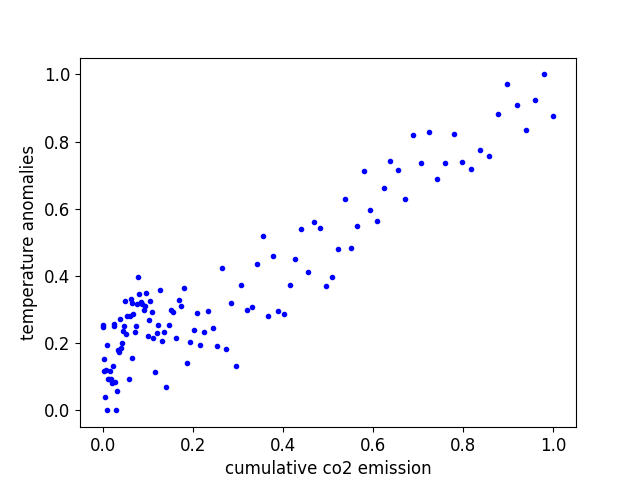
\includegraphics[width=\linewidth]{img/cumulative-co2-temperature.png}
  \caption{}
  \label{fig:cumulative-co2-temperature}
\end{figure}

\newpage
\section{Linear Regresion}

\begin{figure}[h]
  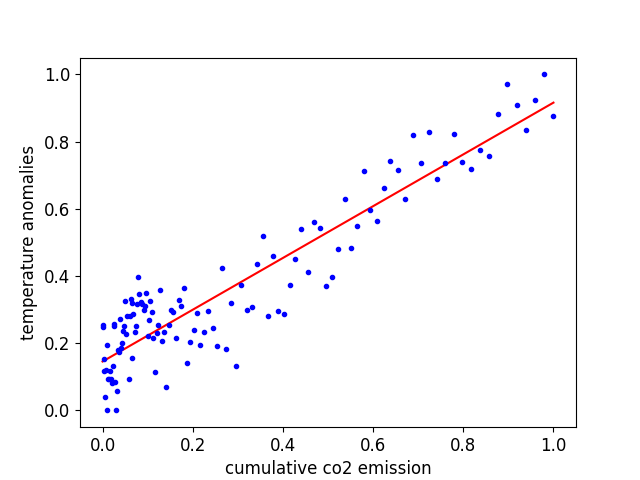
\includegraphics[width=\linewidth]{img/linear-regression.png}
  \caption{Linear Regression model used for temperature anomalies prediction }
  \label{fig:linear-regression}
\end{figure}

\newpage
\section{Polynomial Regression}

\begin{figure}[h]
  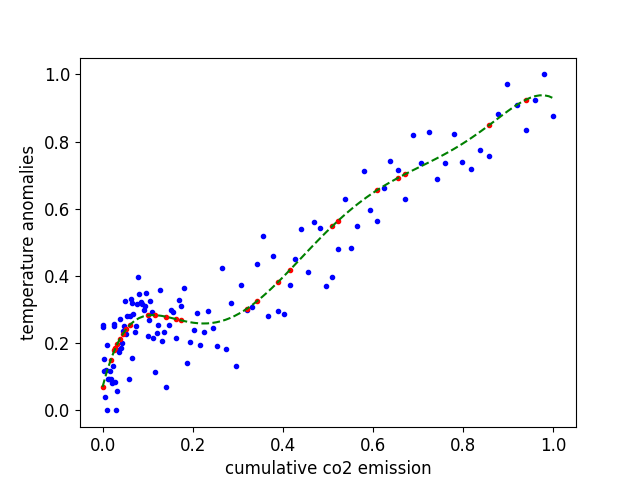
\includegraphics[width=\linewidth]{img/polynomial-regression.png}
  \caption{Polynomial Regression model used for temperature anomalies prediction}
  \label{fig:polynomial-regression}
\end{figure}

\newpage
\section{Ridge Regression}

\begin{figure}[h]
  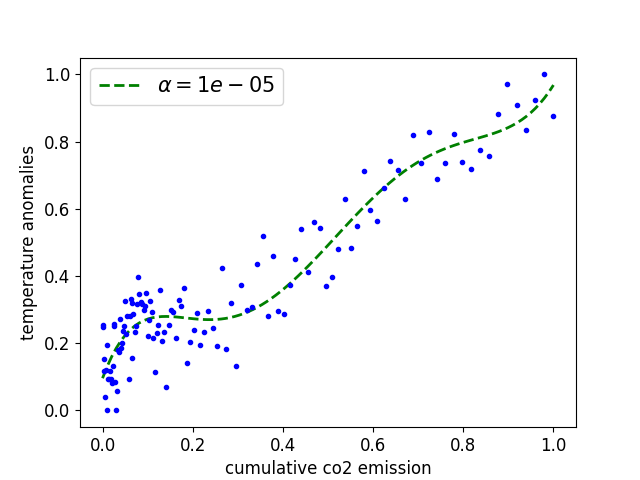
\includegraphics[width=\linewidth]{img/ridge-regression.png}
  \caption{Ridge Regression model used for temperature anomalies prediction}
  \label{fig:ridge-regression}
\end{figure}

\newpage
\section{Lasso Regression}

\begin{figure}[h]
  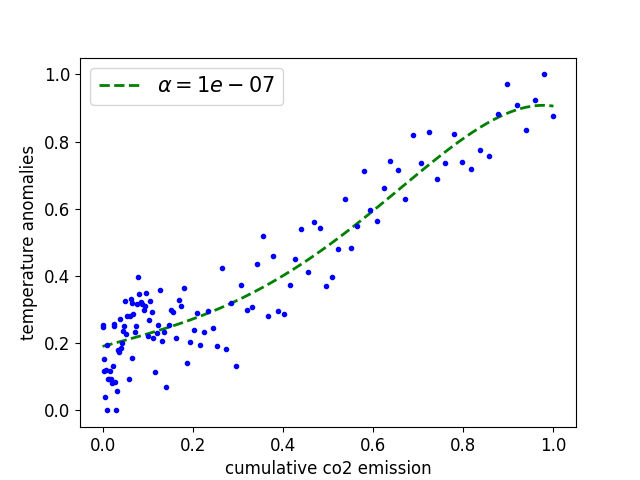
\includegraphics[width=\linewidth]{img/lasso-regression.png}
  \caption{Lasso Regression model used for temperature anomalies prediction}
  \label{fig:lasso-regression}
\end{figure}

\newpage
\section{Gausian Process}

\begin{figure}[h]
  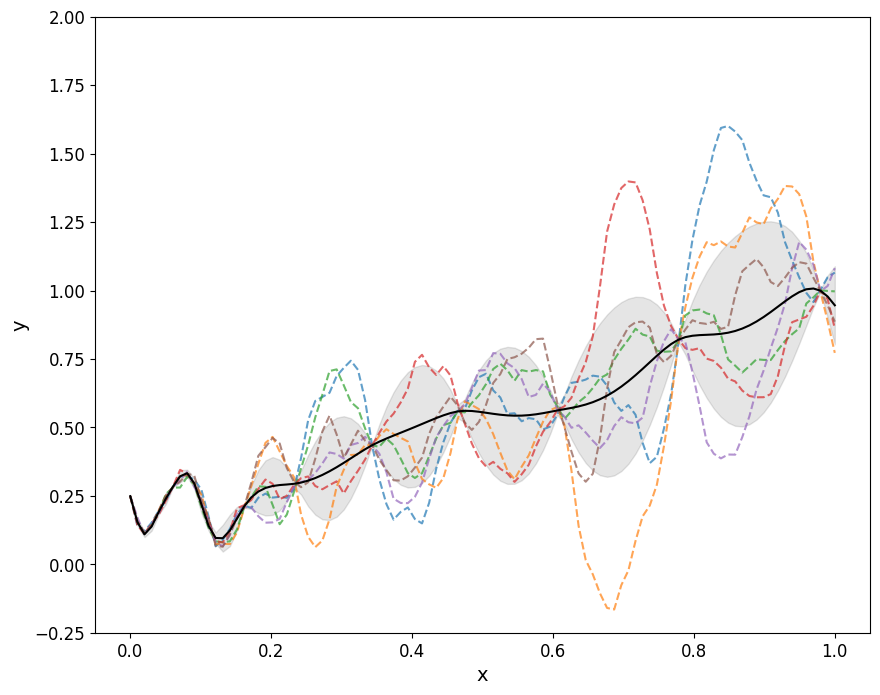
\includegraphics[width=\linewidth]{img/gaussian-process.png}
  \caption{Gaussian Process model used for temperature anomalies prediction}
  \label{fig:gaussian-process}
\end{figure}

\section{Comparision of ML algorithms}

\section{Summary}
